% Options for packages loaded elsewhere
\PassOptionsToPackage{unicode}{hyperref}
\PassOptionsToPackage{hyphens}{url}
%
\documentclass[
]{book}
\usepackage{amsmath,amssymb}
\usepackage{lmodern}
\usepackage{ifxetex,ifluatex}
\ifnum 0\ifxetex 1\fi\ifluatex 1\fi=0 % if pdftex
  \usepackage[T1]{fontenc}
  \usepackage[utf8]{inputenc}
  \usepackage{textcomp} % provide euro and other symbols
\else % if luatex or xetex
  \usepackage{unicode-math}
  \defaultfontfeatures{Scale=MatchLowercase}
  \defaultfontfeatures[\rmfamily]{Ligatures=TeX,Scale=1}
\fi
% Use upquote if available, for straight quotes in verbatim environments
\IfFileExists{upquote.sty}{\usepackage{upquote}}{}
\IfFileExists{microtype.sty}{% use microtype if available
  \usepackage[]{microtype}
  \UseMicrotypeSet[protrusion]{basicmath} % disable protrusion for tt fonts
}{}
\makeatletter
\@ifundefined{KOMAClassName}{% if non-KOMA class
  \IfFileExists{parskip.sty}{%
    \usepackage{parskip}
  }{% else
    \setlength{\parindent}{0pt}
    \setlength{\parskip}{6pt plus 2pt minus 1pt}}
}{% if KOMA class
  \KOMAoptions{parskip=half}}
\makeatother
\usepackage{xcolor}
\IfFileExists{xurl.sty}{\usepackage{xurl}}{} % add URL line breaks if available
\IfFileExists{bookmark.sty}{\usepackage{bookmark}}{\usepackage{hyperref}}
\hypersetup{
  pdftitle={Mappeeksamen},
  pdfauthor={Hermann Moen Kanditatnr.: 111},
  hidelinks,
  pdfcreator={LaTeX via pandoc}}
\urlstyle{same} % disable monospaced font for URLs
\usepackage{longtable,booktabs,array}
\usepackage{calc} % for calculating minipage widths
% Correct order of tables after \paragraph or \subparagraph
\usepackage{etoolbox}
\makeatletter
\patchcmd\longtable{\par}{\if@noskipsec\mbox{}\fi\par}{}{}
\makeatother
% Allow footnotes in longtable head/foot
\IfFileExists{footnotehyper.sty}{\usepackage{footnotehyper}}{\usepackage{footnote}}
\makesavenoteenv{longtable}
\usepackage{graphicx}
\makeatletter
\def\maxwidth{\ifdim\Gin@nat@width>\linewidth\linewidth\else\Gin@nat@width\fi}
\def\maxheight{\ifdim\Gin@nat@height>\textheight\textheight\else\Gin@nat@height\fi}
\makeatother
% Scale images if necessary, so that they will not overflow the page
% margins by default, and it is still possible to overwrite the defaults
% using explicit options in \includegraphics[width, height, ...]{}
\setkeys{Gin}{width=\maxwidth,height=\maxheight,keepaspectratio}
% Set default figure placement to htbp
\makeatletter
\def\fps@figure{htbp}
\makeatother
\setlength{\emergencystretch}{3em} % prevent overfull lines
\providecommand{\tightlist}{%
  \setlength{\itemsep}{0pt}\setlength{\parskip}{0pt}}
\setcounter{secnumdepth}{5}
\usepackage{booktabs}
\AtBeginDocument{\renewcommand{\chaptername}{Kapittel}}
\usepackage{fontspec}
\usepackage{multirow}
\usepackage{multicol}
\usepackage{colortbl}
\usepackage{hhline}
\usepackage{longtable}
\usepackage{array}
\usepackage{hyperref}
\usepackage{booktabs}
\usepackage{wrapfig}
\usepackage{float}
\usepackage{pdflscape}
\usepackage{tabu}
\usepackage{threeparttable}
\usepackage{threeparttablex}
\usepackage[normalem]{ulem}
\usepackage{makecell}
\usepackage{xcolor}
\ifluatex
  \usepackage{selnolig}  % disable illegal ligatures
\fi
\usepackage[]{natbib}
\bibliographystyle{plainnat}

\title{Mappeeksamen}
\author{Hermann Moen Kanditatnr.: 111}
\date{2021-12-02}

\begin{document}
\maketitle

{
\setcounter{tocdepth}{1}
\tableofcontents
}
\hypertarget{realabilitet}{%
\chapter{Realabilitet}\label{realabilitet}}

\hypertarget{introduksjon}{%
\section{Introduksjon}\label{introduksjon}}

Maksimalt oksygenopptak VO2max ble først beskrevet av Hill og Lupton i 1923, og kan defineres som kroppens evne til å ta opp og forbruke oksygen per tidsenhet \citep{bassett2000, hill1923}. Innen toppidrett måles ofte det maksimale oksygenopptaket for å måle utøverens kapasitet opp mot arbeidskravet i den spesifikke idretten, og VO2max kan i så måte også sees på som et mål på den aerobe effekten til utøveren \citep{bassett2000}. I Olympiatoppens testprotokoller benytter de flere definerte hjelpekriterier for å sikre at man faktisk har funnet deltakerens maksimale oksygenopptak \citep{tønnessen2017}. Følgende kriterier er beskrevet; platå i O2 er oppnådd, økning i ventilasjon med utflating av O2 verdi, RER-verdi over 1.10 (1.05 om laktatprofiltest er gjennomført i forkant) og blodlaktat over 8 \citep{tønnessen2017}.

\hypertarget{metode}{%
\section{Metode}\label{metode}}

I forkant av testen ble testpersonen veid uten sko og 300g ble trukket av for vekten av klær. Denne vekten ble brukt i beregningen av maksimalt oksygenopptak (ml kg\textsuperscript{-1} min\textsuperscript{-1}) . For å sikre intern validitet ble deltakerne bedt om å avstå fra anstrengende fysisk aktivitet dagen før test, standardisere måltidet i forkant av test samt avstå fra inntak av koffein under de siste 12 timene før testen \citep{halperin2015}. Både test 1 og 2 ble gjennomført på samme tid på døgnet under standardiserte forhold. Test 2 ble gjennomført 6 dager etter gjennomført test 1. Det ble ikke kontrollert for fysisk aktivitet mellom testdagene.

Det var 11 deltakere(tabell 1) i studien, der deltakerne gjennomførte en 10 minutter lang oppvarmingsprotokoll på tredemøllen (Woodway 4Front, Wisconson, USA), beskrevet for deltakerne i forkant av testen. Denne oppvarmingsprotokollen bestod av fem minutter på 11-13 i Borg 6-20 RPE skala \citep{borg1982}, etterfulgt av 2x1min på starthastighet og stigning med 30 sekund pausene mellom dragene. Siste tre min var også 11-13 i borg på valgfri stigning. Etter oppvarming var det to min pause før testen begynte. Starthastighet (tabell 1) var satt til 8km/t, med stigning på 10.5\% og 5.5\% for henholdsvis menn og kvinner.

VO2max ble målt ved hjelp av en metabolsk analysator med miksekammer (vyntus CPX, mixing­chamber (Vyntus CPX, Jaeger-CareFusion, UK)). Forut for alle tester ble analysatoren gass og volumkalibrert. Analysatoren ble stilt inn til å gjøre målinger hvert 30sek, og VO2max ble kalkulert gjennom å bruke snittet av de to høyeste påfølgende målingene av O2. Underveis i testen mottok alle deltakerne en høylytt verbal oppmuntring fra testleder som var standarisert \citep{halperin2015}. Alle deltakerne gjennomførte også begge testene med samme testleder og med samme personer til stede i rommet for å redusere konfundering \citep{halperin2015}.

For hvert medgåtte minutt av testen ble hastigheten på møllen økt med 1km/t, helt til utmattelse, hvor testen ble avsluttet. Deltakernes hjertefrekvens ble også registrert under hele testen. Når testen ble avsluttet ble deltakerne bedt om å rapportere opplevd anstrengelse ved hjelp av Borg-skala \citep{borg1982}. Maksimal hjertefrekvens under testen ble også registrert. Ett minutt etter avsluttet test ble hjertefrekvens registrert, og det ble målt og analysert blodlaktat (Biosen C-line, EKF Diagnostics, Barleben, Germany).

\providecommand{\docline}[3]{\noalign{\global\setlength{\arrayrulewidth}{#1}}\arrayrulecolor[HTML]{#2}\cline{#3}}

\setlength{\tabcolsep}{2pt}

\renewcommand*{\arraystretch}{1.5}

\begin{longtable}[c]{|p{1.08in}|p{1.02in}|p{1.02in}}

\caption{Deltakeroversikt}\label{tab:Tabell}\\

\hhline{>{\arrayrulecolor[HTML]{666666}\global\arrayrulewidth=2pt}->{\arrayrulecolor[HTML]{666666}\global\arrayrulewidth=2pt}->{\arrayrulecolor[HTML]{666666}\global\arrayrulewidth=2pt}-}

\multicolumn{1}{!{\color[HTML]{000000}\vrule width 0pt}>{\raggedright}p{\dimexpr 1.08in+0\tabcolsep+0\arrayrulewidth}}{\fontsize{11}{11}\selectfont{\textcolor[HTML]{000000}{\global\setmainfont{Arial}{}}}} & \multicolumn{1}{!{\color[HTML]{000000}\vrule width 0pt}>{\raggedright}p{\dimexpr 1.02in+0\tabcolsep+0\arrayrulewidth}}{\fontsize{11}{11}\selectfont{\textcolor[HTML]{000000}{\global\setmainfont{Arial}{Kvinner}}}} & \multicolumn{1}{!{\color[HTML]{000000}\vrule width 0pt}>{\raggedright}p{\dimexpr 1.02in+0\tabcolsep+0\arrayrulewidth}!{\color[HTML]{000000}\vrule width 0pt}}{\fontsize{11}{11}\selectfont{\textcolor[HTML]{000000}{\global\setmainfont{Arial}{Menn}}}} \\

\hhline{>{\arrayrulecolor[HTML]{666666}\global\arrayrulewidth=2pt}->{\arrayrulecolor[HTML]{666666}\global\arrayrulewidth=2pt}->{\arrayrulecolor[HTML]{666666}\global\arrayrulewidth=2pt}-}

\endfirsthead

\hhline{>{\arrayrulecolor[HTML]{666666}\global\arrayrulewidth=2pt}->{\arrayrulecolor[HTML]{666666}\global\arrayrulewidth=2pt}->{\arrayrulecolor[HTML]{666666}\global\arrayrulewidth=2pt}-}

\multicolumn{1}{!{\color[HTML]{000000}\vrule width 0pt}>{\raggedright}p{\dimexpr 1.08in+0\tabcolsep+0\arrayrulewidth}}{\fontsize{11}{11}\selectfont{\textcolor[HTML]{000000}{\global\setmainfont{Arial}{}}}} & \multicolumn{1}{!{\color[HTML]{000000}\vrule width 0pt}>{\raggedright}p{\dimexpr 1.02in+0\tabcolsep+0\arrayrulewidth}}{\fontsize{11}{11}\selectfont{\textcolor[HTML]{000000}{\global\setmainfont{Arial}{Kvinner}}}} & \multicolumn{1}{!{\color[HTML]{000000}\vrule width 0pt}>{\raggedright}p{\dimexpr 1.02in+0\tabcolsep+0\arrayrulewidth}!{\color[HTML]{000000}\vrule width 0pt}}{\fontsize{11}{11}\selectfont{\textcolor[HTML]{000000}{\global\setmainfont{Arial}{Menn}}}} \\

\hhline{>{\arrayrulecolor[HTML]{666666}\global\arrayrulewidth=2pt}->{\arrayrulecolor[HTML]{666666}\global\arrayrulewidth=2pt}->{\arrayrulecolor[HTML]{666666}\global\arrayrulewidth=2pt}-}\endhead



\multicolumn{3}{!{\color[HTML]{FFFFFF}\vrule width 0pt}>{\raggedright}p{\dimexpr 3.13in+4\tabcolsep+2\arrayrulewidth}!{\color[HTML]{FFFFFF}\vrule width 0pt}}{\fontsize{11}{11}\selectfont{\textcolor[HTML]{000000}{\global\setmainfont{Arial}{Verdier\ er\ gitt\ som\ gjennomsnitt\ og\ (Standardavvik)}}}} \\

\endfoot



\multicolumn{1}{!{\color[HTML]{000000}\vrule width 0pt}>{\raggedright}p{\dimexpr 1.08in+0\tabcolsep+0\arrayrulewidth}}{\fontsize{11}{11}\selectfont{\textcolor[HTML]{000000}{\global\setmainfont{Arial}{N}}}} & \multicolumn{1}{!{\color[HTML]{000000}\vrule width 0pt}>{\raggedright}p{\dimexpr 1.02in+0\tabcolsep+0\arrayrulewidth}}{\fontsize{11}{11}\selectfont{\textcolor[HTML]{000000}{\global\setmainfont{Arial}{4}}}} & \multicolumn{1}{!{\color[HTML]{000000}\vrule width 0pt}>{\raggedright}p{\dimexpr 1.02in+0\tabcolsep+0\arrayrulewidth}!{\color[HTML]{000000}\vrule width 0pt}}{\fontsize{11}{11}\selectfont{\textcolor[HTML]{000000}{\global\setmainfont{Arial}{7}}}} \\





\multicolumn{1}{!{\color[HTML]{000000}\vrule width 0pt}>{\raggedright}p{\dimexpr 1.08in+0\tabcolsep+0\arrayrulewidth}}{\fontsize{11}{11}\selectfont{\textcolor[HTML]{000000}{\global\setmainfont{Arial}{Alder\ (år)}}}} & \multicolumn{1}{!{\color[HTML]{000000}\vrule width 0pt}>{\raggedright}p{\dimexpr 1.02in+0\tabcolsep+0\arrayrulewidth}}{\fontsize{11}{11}\selectfont{\textcolor[HTML]{000000}{\global\setmainfont{Arial}{24.5\ (1.29)}}}} & \multicolumn{1}{!{\color[HTML]{000000}\vrule width 0pt}>{\raggedright}p{\dimexpr 1.02in+0\tabcolsep+0\arrayrulewidth}!{\color[HTML]{000000}\vrule width 0pt}}{\fontsize{11}{11}\selectfont{\textcolor[HTML]{000000}{\global\setmainfont{Arial}{23.9\ (1.77)}}}} \\





\multicolumn{1}{!{\color[HTML]{000000}\vrule width 0pt}>{\raggedright}p{\dimexpr 1.08in+0\tabcolsep+0\arrayrulewidth}}{\fontsize{11}{11}\selectfont{\textcolor[HTML]{000000}{\global\setmainfont{Arial}{Vekt\ (kg)}}}} & \multicolumn{1}{!{\color[HTML]{000000}\vrule width 0pt}>{\raggedright}p{\dimexpr 1.02in+0\tabcolsep+0\arrayrulewidth}}{\fontsize{11}{11}\selectfont{\textcolor[HTML]{000000}{\global\setmainfont{Arial}{58.9\ (6.28)}}}} & \multicolumn{1}{!{\color[HTML]{000000}\vrule width 0pt}>{\raggedright}p{\dimexpr 1.02in+0\tabcolsep+0\arrayrulewidth}!{\color[HTML]{000000}\vrule width 0pt}}{\fontsize{11}{11}\selectfont{\textcolor[HTML]{000000}{\global\setmainfont{Arial}{74.8\ (5.55)}}}} \\





\multicolumn{1}{!{\color[HTML]{000000}\vrule width 0pt}>{\raggedright}p{\dimexpr 1.08in+0\tabcolsep+0\arrayrulewidth}}{\fontsize{11}{11}\selectfont{\textcolor[HTML]{000000}{\global\setmainfont{Arial}{Høyde\ (cm)}}}} & \multicolumn{1}{!{\color[HTML]{000000}\vrule width 0pt}>{\raggedright}p{\dimexpr 1.02in+0\tabcolsep+0\arrayrulewidth}}{\fontsize{11}{11}\selectfont{\textcolor[HTML]{000000}{\global\setmainfont{Arial}{166\ (2.99)}}}} & \multicolumn{1}{!{\color[HTML]{000000}\vrule width 0pt}>{\raggedright}p{\dimexpr 1.02in+0\tabcolsep+0\arrayrulewidth}!{\color[HTML]{000000}\vrule width 0pt}}{\fontsize{11}{11}\selectfont{\textcolor[HTML]{000000}{\global\setmainfont{Arial}{180\ (3.1)}}}} \\

\hhline{>{\arrayrulecolor[HTML]{666666}\global\arrayrulewidth=2pt}->{\arrayrulecolor[HTML]{666666}\global\arrayrulewidth=2pt}->{\arrayrulecolor[HTML]{666666}\global\arrayrulewidth=2pt}-}



\end{longtable}

\hypertarget{resultater}{%
\section{Resultater}\label{resultater}}

Deskriptive data for disse deltakerne er vist i Tabell 1, i Figur 1 kan man se forskjellen mellom test 1o og 2 fordelt på kjønn. Det typiske målefeilet (typical error, \citep{hopkins2000}) fra test 1 til test 2 er utregnet til å være 4.04\%.

\begin{figure}
\centering
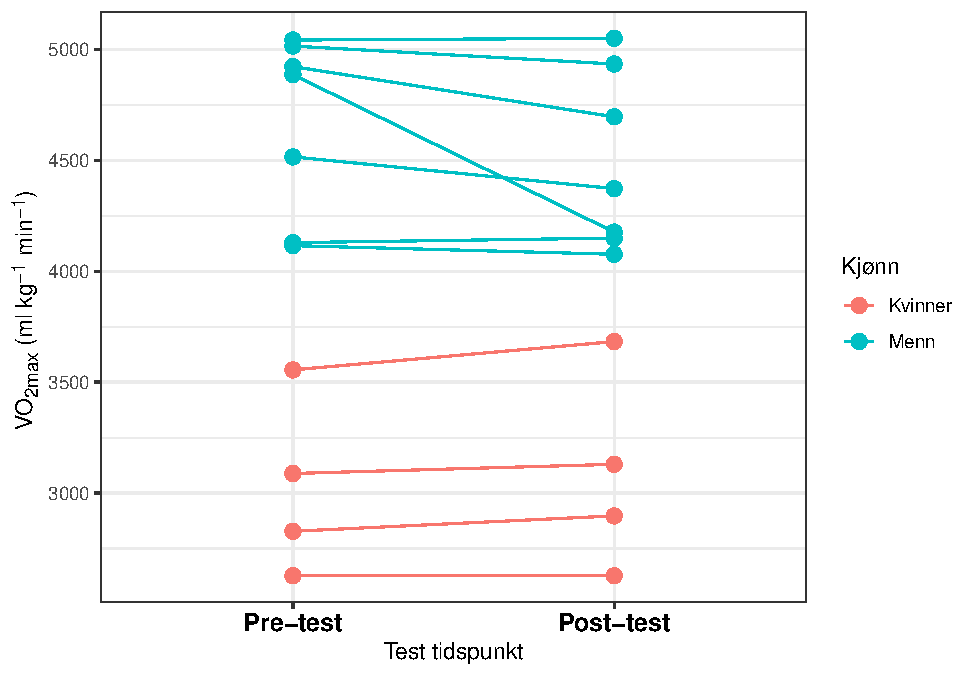
\includegraphics{_main_files/figure-latex/Figur-1.pdf}
\caption{\label{fig:Figur}Figuren viser forskjellen i VO2max(ml/min) i test 1 og test 2}
\end{figure}

\hypertarget{diskusjon}{%
\section{Diskusjon}\label{diskusjon}}

4,04\%

Resultatet i vår realibiltetsstudie er funnet av typefeilen på 4,04. Ettersom testing av maksimalt oksygenopptak er en test som gjennomføres til utmattelse, vil man kunne forvente en viss variasjon i testresultatene ettersom opplevd anstrengelse kan påvirkes av flere ulike variabler \citep{halperin2015}. For å redusere støy vil flere faktorer være nyttig å ta hensyn til under slik testing. Som nevnt i metoden vil standardisering av matinntak, koffeininntak, utstyr og tidspunkt for gjennomføring av test være med på å kunne sikre intern validitet i resultatene. Eksempler er deltakernes kjennskap til testen, verbal oppmuntring og personer tilstede under testen er andre faktorer som potensielt kan bidra til støy \citep{halperin2015}. Felles for alle faktorer er at graden av påvirkning på resultatene muligens reduseres ved hjelp av en standardisert testprotokoll. Deltakerne - og testlederne, sin kjennskap til testen er en annen faktor som trolig påvirker resultatene i vårt prosjekt. I dette tilfellet fantes det enkelte deltakere som hadde gjennomført en liknende test flere ganger, og en kan da forvente en mindre grad av variasjon mellom resultatene på test 1 og test 2, sammenlignet med de deltakerne som gjennomførte testen for første gang på pretest. Dette fordi kjennskapen og kunnskapen de tilegnet seg på pre-test, trolig spiller inn på testresultatene. Typefeilen på 4.04\% kan også tyde på at enkelte av disse resultatene kan være utsatt for støy av ulik sort \citep{hopkins2000}.

Grunnen til at vi snakker om typefeil er at når vi ønsker å måle påvirkningen av trening på en gruppe individer er det viktig å kunne si noe om hva som er endring og hva som er støy (målefeil). Desto mindre støy en test innebærer jo bedre er målingen. Målet som brukes er typefeil. Hva som danner denne variasjonen som representeres ved typical error er multifaktorelt, men hoveddelen er som oftest biologisk \citep{hopkins2000}.

For å måle typefeil har vi brukt within subject deviation metoden. Denne metoden påvirkes ikke av at gjennomsnittet endrer seg fra test til test \citep{hopkins2000}. Data for målinger i VO2max fra fem sertifiserte Australske laboratorier fastslo ett gjennomsnitt på 2.2\% for typefeil \citep{halperin2015}. Data fra det Australske institutt for sport har også fastslått at en typefeil på omtrent 2\% er riktig for både maksimal og submaksimal O2 \citep{clark2007, robertson2010, saunders2009}. Dette indikerer at med godt kalibrert utstyr og med utøvere som er godt vant med testingen vil en typefeil på 2\% for det biologiske, og analytiske være riktig \citep{halperin2015}. Vår typefeil på 4.04\% kan derfor tenkes å være et bilde hvordan det kan se ut med få deltakere, med ulikt utgangspunkt, men også uten skikkelig standardisering av treningshverdagen i forkant av testene. Det kan også tenkes at med et varierende nivå hos deltagerne kan enkelte oppleve en treningseffekt av test 1. Samtidig som andre kanskje ble slitne av å få en test inn i treningshverdagen.

\hypertarget{labrapport---cdna-synthesis-using-superscript-iv-and-general-qpcr}{%
\chapter{Labrapport - cDNA synthesis using Superscript IV and general qPCR}\label{labrapport---cdna-synthesis-using-superscript-iv-and-general-qpcr}}

\hypertarget{formuxe5l}{%
\section{Formål}\label{formuxe5l}}

RNA-overflodsanalyse er gjort ved hjelp av syntese av komplementært DNA fra enkelttrådet RNA. Vi ønsker å amplifisere opp bestemte proteiner ved hjelp av bestemte primere og qPCR. Vi ønsker å få frem en cQ-verdi for å kunne evaluere gen-opphopningen, og sammenlikne mål-genene med referanse gener.

\hypertarget{metode-1}{%
\section{Metode}\label{metode-1}}

Vi hentet cDNA fra 3 forsøkspersoner. Dette er cDNA hentet fra testene som ble gjennomført i uke 0 og uke 2. Alle prøver er fra venstre ben. Det ble laget en 5 fortynningsserier fra disse prøvene. Dette ble fortynnet ved hjelp av DEPC-behandlet vann, i følgende serie 1:10, 1:50, 1:250, 1:1250, 1:6250, 1:31250, 1:156250. Vortex ble brukt mellom hver fortynningsfase.

Det ble derreter laget sju forskjellige master mixer ved hjelp av 3 referansegener (REEP5, CHMP2A, B2M) og 4 målgener (MyHC I, 2A, 2X, rRNA 475). Mastermix bestod av 5 µl sybr green, 1 µl valgt gen, 2 µl DEPC-behandlet vann , 2 µl fortynnet cDNA. Deretter ble det fylt 71 brønner i en qPCR-reaksjonsplate ed henholdsvis 2 µl prøve, og 8 µl med mastermix. Reaksjonsplaten med brønner ble dekt med plastfilm, og sentrifugerte 1 minutt på 1200 omrdreininger (rpm), før PCR protokoll ble gjennomført.

En PCR protokoll ble på forhånd forberedet i QuantStudio5. PCR protokollen bestod av 50 grader i 2 minutter, og 95 grader i 2 minutter, før den kjørte 40 sykluser bestående av 1 sekund på 95 grader celsius, og 30 sekunder på 60 grader celsius.

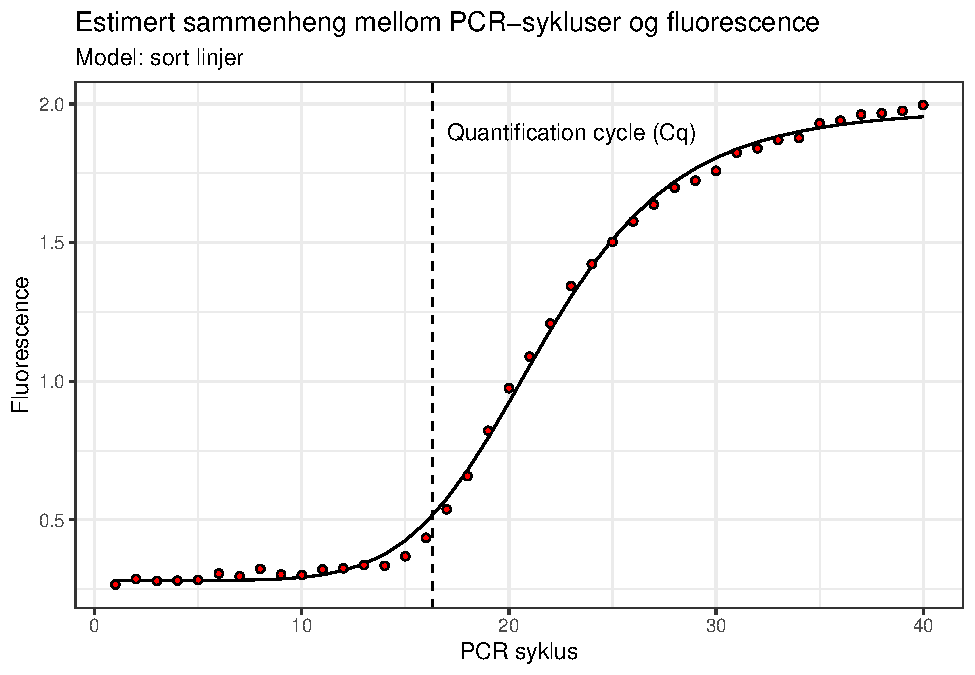
\includegraphics{_main_files/figure-latex/unnamed-chunk-3-1.pdf}

\hypertarget{resultater-1}{%
\section{Resultater}\label{resultater-1}}

Modellen viser sammenhengen mellom antall sykluser og fluorescence. Flere PCR-sykluser gir flere kopier, og dermed også en økt konsentrasjon i prøven. På denne måten kan vi bruke fluorescence til å si noe om hvor mange sykluser som må til for å oppnå en bestemt terskelverdi(Cq-verdi). Med primerne vi benyttet i forsøket var det ønskelig med et sted mellom 10 og 40 sykluser for å sikre at vi oppnådde terskelverdien. Det ble derfor kjørt 40 sykluser.Ved flere sykluser øker trolig sannsynligheten for falske positive.

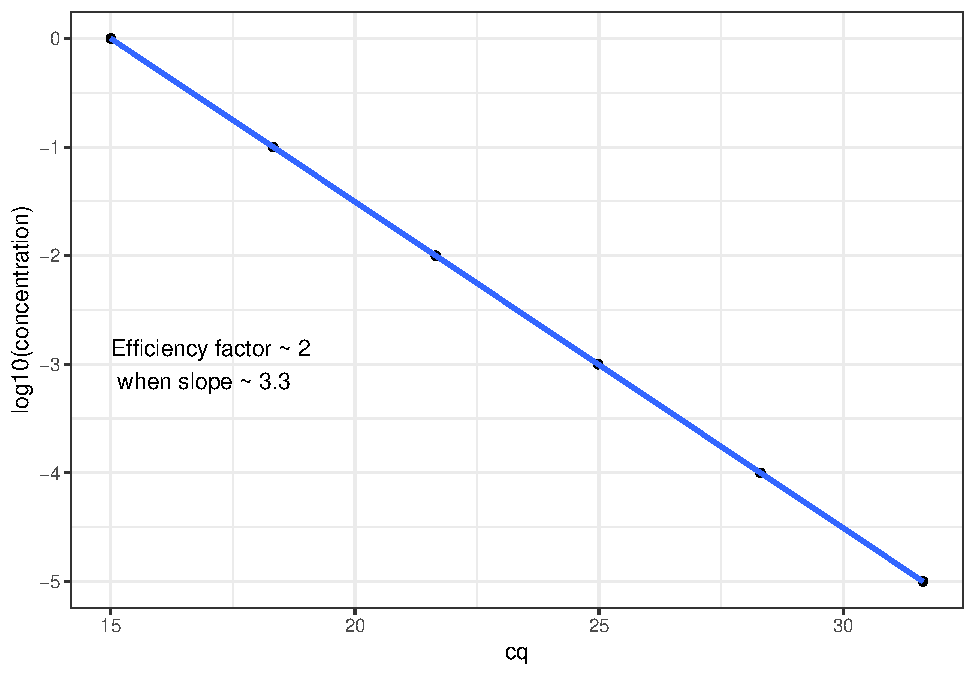
\includegraphics{_main_files/figure-latex/unnamed-chunk-4-1.pdf}

\begin{figure}
\centering
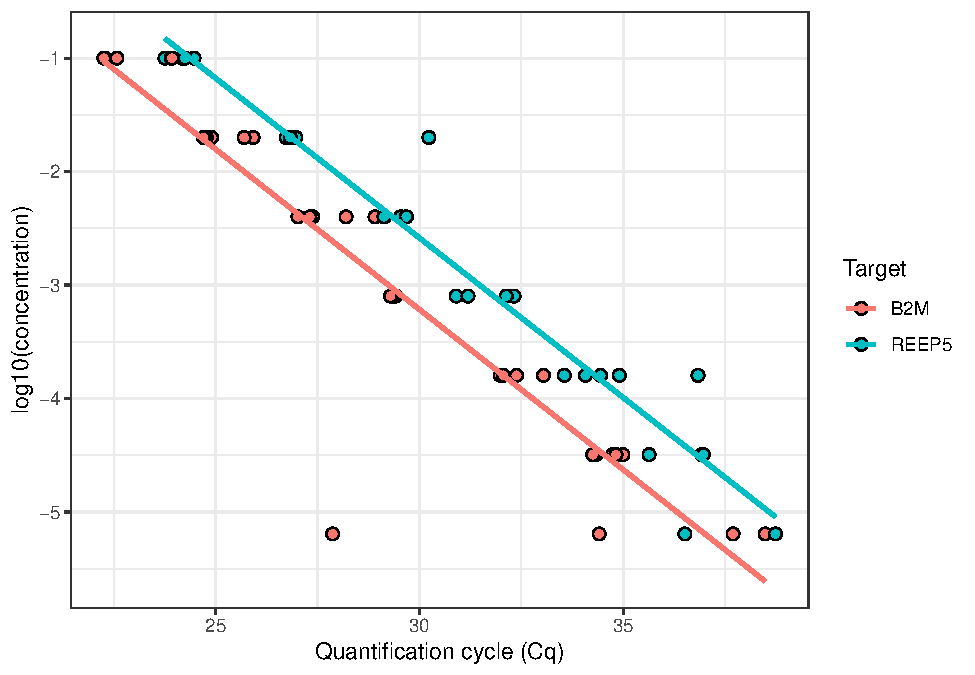
\includegraphics{_main_files/figure-latex/unnamed-chunk-5-1.pdf}
\caption{\label{fig:unnamed-chunk-5}Efficiency calculations made from serial dilution of cDNA}
\end{figure}

\hypertarget{diskusjon-1}{%
\section{Diskusjon}\label{diskusjon-1}}

Cq-verdien sier noe om hvor mange PCR-sykluser som trengs for å detektere ulike målgen\citep{kuang2018}. En høyere Cq-verdi indikerer altså at mengden RNA må dobles flere ganger for å detektere en terskelverdi av target. En lavere Cq-verdi indikerer at terskelverdien oppnås ved færre PCR-sykluser, altså at konsentrasjonen av target er høyere. En lavere Cq-verdi ved uke 2, sammenlignet med uke 0(baseline) som i forsøket, indikerer høyere konsentrasjon ved uke 2 enn ved uke 0. Dermed en effekt av intervensjonen, avhengig av funksjonen til målgenet vi underøkser.

\hypertarget{vitenskapsteori}{%
\chapter{Vitenskapsteori}\label{vitenskapsteori}}

\hypertarget{falsifikasjon}{%
\section{Falsifikasjon}\label{falsifikasjon}}

Falsifiseringsprinsippet Karl Raimund Popper (1902-1994), var en Østerisk-Britisk filosof. Popper hadde siden høsten 1919 bearbeidet spørsmålet om hva som skulle til for å kunne dannet et skille mellom vitenskap og pseudo-vitenskap. På den tiden(starten av og et stykke inn på 1900tallet) var det en aksept for at skilnaden mellom vitenskap og pseudo-vitenskap, var den empiriske fremgangsmetoden \citep{popper2002}. Den empiriske fremgangsmetoden går fra observasjoner, eller eksperimenter til å danne teorier ved hjelp av induktive argumenter. Et induktivt argument bygger på at premissene som er satt er sanne, og ved nok observasjoner av disse premissene, vil konklusjonen sannsynligvis være sann, eller man kan si at man har styrket bekreftelse av en teori. Denne tankerekkefølgen ble kritisert av David Hume (1711- 1776) allerede på 1700tallet. Hume stilte spørsmål for hvordan man kan slå fast at induksjon er pålitelig, og svaret ble ved hjelp av et argument. Hvilket argument skulle brukes? Induktiv metode kan ikke garanteres for ved et deduktivt argument, da det ikke finnes et deduktivt argument for at induksjon vil fungere i fremtiden. Et induktivt argument bygger på erfaringer, men kan heller ikke slå fast induksjonens sikkerhet. Dette var kronglete å holde styr på i hodet, men var et fundamentet i kritikken av induksjonismen langt inn på 1900tallet.

Popper som i utgangspunktet var ute etter å skille vitenskap fra pseudo-vitenskap viste om denne svakheten ved induktive argumenter som var det som var det opprinnelige skille. Ved hjelp av datidens største og mest fremgangsrike vitenskapsteorier lette Popper etter forskjeller. Einsteins relativitetsteori, marx historiske teorier, Freuds psyko-analyser, og Alfred Adlers individuelle psykologi var de mest omtalte teoriene på den tiden. Når han etter hvert oppdaget at flere av punktene i de forskjllige teoriene ble bekreftet, ble han også mens tiden gikk mindre og mindre imponert av Marx, Freud og Adler. Det var her han startet å se etter forskjeller. De andre teoriene hadde mange bekreftelser, og hvert eneste tilfelle kunne på en eller annen måte forklares ved hjelp av teoriene. Einsteins relativitetsteori kunne derimot motsies ved hjelp av en eksakt måling. Ut av dette vokste Poppers falsifiserbarhetskriterium \citep{popper2002}.

Falsifiserbarhetskriteriumet vokste altså frem av at en teori ikke burde bekreftes, men avkreftes, eller falsifiseres som det kalles vitenskapelig. Teorien må derfor være så konkret at den kan måles, og dermed falsifiseres. Et eksmpel kan være: «det kommer til å regne i morgen». Dette utsagnet vil i løpet av morgendagen kunne falsifiseres, hvis det blir oppholdsvær. Om det skulle regne, vil det komme en ny morgendag, der teorien kan falsifiseres. Dette vil skille pseudo-vitenskap og vitenskap i og kalles for Poppers demarkasjonskriterium. Vitenskap vil derfor være alle teorier som kan falsifiseres. Når noe er falsifisert vil det vokse frem en ny falsifiserbar teori, og vitenskapen som en enhet vil etter hvert nærme seg en sannhet. Med dette kriterium mente også popper at induksjonsproblemet også var løst. Dette mente han ved at alle vitenskapelige teorier er deduktive argumenter som falsifiserer, og at vitenskapen dermed ikke behøver bruke induktive argumentasjon. Denne tankerekkefølgen gjør at man ikke kan stole på at noen ting vil være sant, eller ikke engang at det kan argumenteres for at det er sannsynlig å være sant.

Dette er en av punktene som kritiseres av andre filosofer. Altså er det ikke mulig å si at noe er mer sant en annet. Popper kritiseres av andre av at det ikke er forskjell på godt bekreftede og dårlig bekreftede teorier. Det gjør også det mulig å sette opp nye teorier, eller endre teorier sånn at en teori ikke er falsifisert, da man ikke har noen form for hierarki over hvilke teorier som er best bekreftet. Et annet argument som ofte trekkes frem i denne sammenhengen er at det ikke trenger å være et klart skille mellom hva som er ekte vitenskap, og hva som er pseudo-vitenskap. Det vil i mine øyne ikke være så viktig da hvor godt noe er bevist eller bekreftet bør veie tyngre enn at det er formulert en hypotese som kan motsies. I mine øyne er en god vitenskapelig teori noe som er godt bekreftet. Et argument mot denne definisjonen på god vitenskapelig teori, er at den er en lite konkret og veldig vag definisjon, som er vanskelig å standardisere, og dermed dårlig i praksis. Denne definisjonen på en god teori, betyr at i praksis at teorien er bygget i bunn på induktive argumenter. Det er flere forskjellige metoder å benytte seg av induktiv argumentasjon, fire kjente måter er: Hypotetisk deduktiv metode, naiv induktivisme, abduksjon, og bayesianisme\\

\hypertarget{hd-metoden-og-abduksjon}{%
\section{HD-metoden og abduksjon}\label{hd-metoden-og-abduksjon}}

En av de som støttet induktiv argumentasjon for vitenskapelig teorier var Carl Hempel (1905- 1997), han var naturlig nok (delte nesten et helt århundre sammen, med motsatte meninger) en av Poppers kritikkere. Han kritiserte også naiv induktivisme, som baserte seg rundt to påstander. Den første er at en teori kan støttes induktivt når den kan trekkes ut fra et utvalg, og den andre er at teorien da bør formuleres etter at alle dataene er innsamlet. Hempel hang seg spesielt opp i det siste og mente at det var umulig å trekke noen konklusjoner før tidens slutt, da det alltid vil dukke opp nye data. Ei heller ville det være mulig å innhente all data som eksisterer i dag. \citep[s. 11]{hempel1966} Hempel var av en annen oppfatning av hvordan en teori kunne bekreftes. Hempel mente dette var den hypotetsik deduktive metoden.\\

Den hypotetisk deduktive metoden baserer seg på fire steg. Det første steget er steget der det dannes eller formuleres en hypotese, teori etc. Dette steget gjøres ved hjelp av et «educated guess», eller «utdannet gjetning» som oversettelsen blir. Det neste steget er deduksjon, som i praksis betyr å utlede empiriske konsekvenser. Her legges grunnlaget for de neste to stegene da disse empiriske konsekvensene deduseres. I steg tre blir disse deduserte empiriske konsekvensene testet ut, som dirkete leder til steg fire. Hvis disse empiriske konsekvensene viser seg å være sanne er denne teorien induktivt bekreftet, eller induktivt styrket bekreftelse av teorien \citep[s.12-13]{hempel1966}. Den hypotetisk deduktive metoden kan forklares som en vei med to kjøreretninger, fra data til teori går det induktive argumentet, som er bygd på deduktivt argument som går motsatt vei, altså fra teori til data. Problemet knyttet til Hypotetisk deduktiv metode er at ikke alt kan deduseres, samt at enklere teorier kan passe like bra eller bedre. Om man følger Ockhams barberkniv ønsker man å skjære bort alt unødvendig, da den enkleste teorien som oftetst vil være rett.

Abduksjon er en liknende modell til den hypotetsik deduktive metoden, men har et par vir og vendinger som gjør dem klart forskjellige allikevel. Der den hypotettisk deduktive metoden vil undersøke en hypotese kan en ved hjelp av abduksjon undersøke flere teorier.Så lenge teoriene gir en forklaring på fenomenet kan de sammenliknes, og evalueres. Deretter slutte seg til den beste teorien som forklarer et fenomen. Er det ingen annen teori som gir like god eller bedre forklaring, har teorien induktivt styrket bekreftelse eller er bekreftet.Dette kan oppfattes som subjektivt, for hva er egentlig en bedre forklaring når begge terorier forklare fenomenet. I Abduksjon vil enkelhet tas hensyn til og hvis tre teorier forklarer det samme fenomenet vil det enkleste induktivt bekreftes.

\hypertarget{replikasjonskrisen}{%
\section{Replikasjonskrisen}\label{replikasjonskrisen}}

En viktig faktor i vitenskapens unione søken mot et bedret kunnskapsbilde er åpenhet, det skal kunne testes av andre forskere at man får samme data fra samme forsøk. Dette er for å kunne styrke eller svekke et fenomens teori, og kanskje kunne oppdage en ny teori. For at dette skal kunne skje må forskningen være repliserbar. Dette er ikke vært gjennomført godt nok i de siste årene. Et økt fokus har gjort at det har kommet tall på problemene. 1576 forskere fikk spørsmål om det var en signifikant krise når det kommer til reproduserbarhet i forskning, i en undersøkelse for journalen Nature, der 52\% av deltakerne var enige i det \citep{Baker2016}.\\

Forklaringen på hva som står bak denne krisen er bestående av en hel haug med små og store bidragsytende faktorer. Den minst beskuende og tillitsfulle forklaringen ligger i statistikken. Sånn at replikasjonskrisen kan være et produkt av to statstiske faktorer. De fleste hypoteser vi tester er usanne, og nivået for statistisk signinikans er for lavt (p=\textless0,05).Dette forklarer bird ved hjelp av basefrekvensfeilen. Birds forklaring på replikasjonskrisen er at basefrekevnsfeilen vil oppstå når man trekker en slutning på et fenomen basert på en undersøkelse, men ikke hensyntar hvor normalt fenoment er i utgangspunktet. Han mener dette er en av grunnene for at det er så store problemer med å replisere studier.

Det forekommer tvilsomme forskningspraksiser, som f.eks tuklinger med data, p-hacking, fjerning av materiale. Det er mange små studier, som fører til lav statistisk styrke. Det publiseres ikke like ofte studier med kjedelige eller negative resultater \citep{bird2020}. Det er også kraftig motivasjon for å få frem data med overraskende, eller nyttig resultat, som kan føre til at det blir gjort små ting som gjør at data ikke kan repliseres\citep{romero2017}.\\

For meg høres dette ut som et kombinert problem. Kanskje er verden sånn at vi ikke presterer den beste forskningen i ett frittstående konkurransebasert miljø. Det kan være at det er enklere å få navnet opp og frem med noe kontroversielt enn med noe som støtter en allerede eksisterende teori. I det idrettsvitenskaplige fagfeltet er det ofte små utvalg i intervensjoner som gjennomføres, og med relativt kort varighet i forhold til adaptasjonene som skal måles på, som gjør at det krever at mye skal stemme for å få et signifikant resultat, som kan forsterke publikasjonsskjevheten, og dårlig forskningspraksis for å kunne få signifikante resultater.

\hypertarget{study-designs}{%
\chapter{\texorpdfstring{\textbf{Study Designs}}{Study Designs}}\label{study-designs}}

I denne opggaven om studie design vil jeg bruke QALMRI metoden \citep{brosowsky2020} for å bryte ned artiklene fra fem forskjllige originale studier som undersøker det samme i et vitenskapelig område. De utvalgte studiene for denne analysen er \citep{johnsen2021}, \citep{brigatto2019}, \citep{gentil2018}, \citep{saric2019}, og \citep{lasevicius2019}.

\hypertarget{hva-undersuxf8ker-disse-studiene}{%
\section{Hva undersøker disse studiene?}\label{hva-undersuxf8ker-disse-studiene}}

Den overordnede tematikken i mine utvalgte studier er trenigsfrekvens, og hvilke påvirkninger den har på adaptasjonene. Treningsfrekvens beskrives i litteraturen som hvor mange treningsøkter som gjennomføres i en gitt tidsperiode, men også som hvor mange ganger en muskelgruppe blir trent i løpet av en periode eller hvor mange økter som blir gjennomført \citep{kraemer2004, schoenfeld2016}. Alle disse studiene kontrollerer volum på den nevnte definisjonen.

Studiene utforsket tilpasningene til styrketrening med forskjellig antall treningsøkter med likt ukentlig treningsvolum. De ønsket altså besvare hvilken treningsfrekvens som ga de beste tilpassningene \citep{johnsen2021, brigatto2019, gentil2018, saric2019, lasevicius2019}.

\hypertarget{hva-kan-forklare-resultatene}{%
\section{Hva kan forklare resultatene?}\label{hva-kan-forklare-resultatene}}

Alle disse studiene hadde en forklaring for hvorfor studien ble gjort formulert som et form for spørsmål, men det var også hypoteser i introduskjonen. I introduksjonen forklares bakgrunnen for studien, og hvilke funn som kan forventes basert på tidligere fagfellevurdert forskning. For eksempel skrev \citep{brigatto2019} at basert på tidligere forskning ville de forvente bedre adaptasjoner i gruppen som trente 2x 8 sett per uke enn i gruppen som trente 1x 16 set per uke. Dette skilte seg fra studiene som sammenlinket høyere frekvenser. \citep{saric2019} som sammenlinket 3 vs 6 økter per uke med likt ukentlig treningsvolum, formulerte en hypotese om at det ville være like adaptasjoner, basert på studiens design og tidligere forskning med kontrollert ukentlig volum og liknende protokoller. Dette er en styrke i alle studiene, og de fokuserer på liknende intervensjoner, og forklarer begrensningene når de sammenlikner med mindre liknende protokoller. Det kan også være andre ting en den tenkte årsaksammenhengen som kan forklare hypotesen, det kan være bias, sjanse, virkning-årsak, og forvirrende faktorer \citep{hulley_2013}

\hypertarget{hvilken-sammenheng-har-hypotese-med-eksisterende-litteratur-i-studiene}{%
\section{Hvilken sammenheng har hypotese med eksisterende litteratur i studiene?}\label{hvilken-sammenheng-har-hypotese-med-eksisterende-litteratur-i-studiene}}

Logikken i veien til en hypotese eller spørsmål i disse studiene som undersøker effekten av forskjellige treningsfrekvenser baseres i alle disse studiene på tidligere evidens fra andre fagfellevurderte artikler\citep{brigatto2019, gentil2018, johnsen2021, saric2019, lasevicius2019}. Selv om disse studiene undersøker det samme overordnede spørsmålet, gjør de metodiske forskjellene i studiene at formuleringen av hypotesene blir forskjellig som vist i avsnittet over.

Studiene som har undersøkt høyere frekvenser opp mot hverandre \citep{johnsen2021, saric2019} bruker også den samme vitenskaplige evidensen for å komme frem til sin hypotese som studiene som undersøker lavere frekvenser\citep{brigatto2019, gentil2018, lasevicius2019}. En styrke ved Studiene med høyere frekvenser,er at de i tillegg legger vekt på at det er mindre forsket på, og støtter seg derfor på generell evidens om at likt treningsvolum gir like adaptasjoner\citep{johnsen2021, saric2019}.

\hypertarget{hvilke-forskjeller-er-det-i-de-metodiske-valgene-i-studiene}{%
\section{Hvilke forskjeller er det i de metodiske valgene i studiene?}\label{hvilke-forskjeller-er-det-i-de-metodiske-valgene-i-studiene}}

Alle disse studiene har en lik type design. Studiene som undersøkes kalles longituelle studier. Den ekspermientielle tilnærmingen baserer seg på to randomiserte grupper, som følger to forskjellige forutbestemte protokoller for å se om det gir utslag på pre til post test resultater. Randomiserte kontrolerte forsøk som dette kalles, gjøres for å undersøke en bestemt variabel, og er en streng rigid metode for å finne årask-virkning mellom variabelen og utfallet \citep{sibbald1998}. Dette gjøres ved at en gruppe mottar en type behandling eller trening, og sammenliknes opp mot en annen gruppe som ofte kalles kontrollgruppe, som enten mottar annen behandling/trening, eller ingenting. Randomiserte kontrolerte studier er dyre, krever mere tid, men gir til gjengjeld, sammen med tidligere evidens, bedre forklaring på årsak-virkning enn kohort studier og case-controll design\citep{hulley_2013}.

Treningsfrekvensen er variabelen som undersøkes i disse studiene, og basert på tidligere forskning må de ha et likt totalt treningsvolum i begge gruppene, for å kunne undersøke effekten av frekvensen best mulig. Derfor er måten de gjennomfører randomisert kontrolerte studier her, ved å dele en gruppe mennesker fra samme segment, gjennom en like lang treningsintervensjon, med likt ukentlig volum, men forskjllig frekvens. Dette er hensyntatt og er en styrke i alle studiene. Det som varierer i disse studienes metoder er varighet på intervensjon, testmetoder, antall deltakere, frekvens som nevnt tidligere og til en viss grad hvilket samfunns segment forsøkspersonene tilhører.

Alle studiene har beskrivende data på sin deltaker masse. \citep{saric2019} sin studie hadde en deltaker masse bestående av 30 styrketrente menn, (gjennomsnitt+Standardavvik) alder = 22.6 +- 2.1 år, høyde = 183,1+-6,0cm, og kroppsvekt = 87,2+-11,6kg. Dette er en styrke med denne studien, da det er et froholdsvis høyt nivå på deltakerne, og et relativt stort utvalg sammenliknet med andre studier. Svakheten med denne studien er at den bare hadde en treningsintervensjon med varighet på 6 uker.

Stuiden til \citep{saric2019} undersøkte muskelstyrke ved hjelp av 1RM, muskulær utholdenhet med RM på 60\% av 1RM, og muskeltykkelse ved hjelp av ultralyd. De samme testene pre og post ble gjort i studien til \citep{brigatto2019}, men som testet lavere frekvenser mot hverandre, og med en lengere intervensjon, som er en av styrkene i den studien. Disse studiene undersøkte begge frekvens på styrketrente menn, men med såpass store metodiske variasjoner at hypotesene er forskjellige.

I alle studiene brukes det flere forskjellige statistiske tester. Frekventiske tester er brukt i samtlige, som feks Shapiro-wilk test \citep{brigatto2019, johnsen2021, lasevicius2019}, t-test \citet{brigatto2019}, og 2x2 repetert ANOVA \citep{brigatto2019, johnsen2021} . Den andre måten er å estimmere en hypoteses sansynlighet ved hjelp av bayesisk sansynlighet, som i tillegg til frekventistisk statestikk blir gjort i \citep{saric2019}.

Alle de evaluerte studiene har også beregnet effekt størrelse fra pre-post test resultatene \citep{brigatto2019, gentil2018, johnsen2021, saric2019, lasevicius2019}.

\hypertarget{hva-er-resultatene-og-konklusjonene}{%
\section{\texorpdfstring{\textbf{Hva er resultatene og konklusjonene}}{Hva er resultatene og konklusjonene}}\label{hva-er-resultatene-og-konklusjonene}}

I alle studiene besvares hypotesen, men det presiseres også at det trengs mer forskning på området for å kunne konkludere. Det gis også forklaringer på betydningen av metodiske svakheter i studiene som for eksempel små utvalg, og kort varighet som . Disse studiene viser også at den metodiske utformingen er viktig da frekvensens påvirkning kan gi signifikant p-verdi i en type studie, med lavere frekvenser som sammenliknes, men ikke i andre. Derfor er også konklusjonene litt forskjellige, og gjelder kun for frekvensene som sammenliknes, og ikke treningsfrekvens generelt \citep{johnsen2021, brigatto2019, gentil2018, saric2019, lasevicius2019}.

\hypertarget{huxf8yere-treningsvolum-leder-til-bedre-styke-og-muskelvekst-i-underekstremiteter-hos-utrente}{%
\chapter{Høyere treningsvolum leder til bedre styke og muskelvekst i underekstremiteter hos utrente}\label{huxf8yere-treningsvolum-leder-til-bedre-styke-og-muskelvekst-i-underekstremiteter-hos-utrente}}

\hypertarget{introduksjon-1}{%
\section{Introduksjon}\label{introduksjon-1}}

Styrketrening er anerkjent som en god metode til å forbedre muskelstyrke, evnen til kraftproduksjon, skape muskelhypertrofi, samt forbedre en rekke helsemarkører \citep{kraemer2002}. Kunnskap om hvordan man best tilrettelegger styrketrening for å opnå de ønskede adaptasjonene viktig, da styrketrening består av en rekke variabler som kan manipuleres ut ifra behov og gi ønsket adaptasjon \citep{kraemer2004, bird2005}. Disse variablene som kan påvirke adaptasjoner er volum, frekvens, pauselengde, øvelsesutvalg, og øvelsesrekkefølge \citep{American2009}.

Treningsvolum og den tilknyttede dose-reponsen er således interesant for å øke effektiviteten av trening. De akutte responsene på forskjllige treningsvolum er undersøkt, og myofibrililær muskelproteinsyntesen ble signifikant økt når deltakere gjennomførte 3set på 70\% av 1rm, vs 1 sett målt 5 og 29 timer etter trening \citep{burd2010}. Når det kommer til lengere varende intervensjonsstudier er det konflikt relatert til treningsvolumets påvirkning. Noen studier har vist signifikant bedre tilpassninger til høyere volum enn lavere volum \citep[ ]{rønnestad2007, starkey1996, radaelli2015}. Andre studier har vist at det ikke skiller seg i tilpassninger til styrketrening med forskjellig volum\citep{bottaro2011, galvao2005, mcbride2003}. Treningssadaptasjoner er avhengig av en rekke biologiske variabler. Målet med denne studien er å fjerne så mye biologisk påvirkning som mulig og undersøke effekten av volumet alene så godt som mulig.

\hypertarget{deltakere-og-studieoversikt}{%
\section{Deltakere og studieoversikt}\label{deltakere-og-studieoversikt}}

Deltakerne i denne studien bestod av ikke røykende kvinner og menn mellom 18 og 40år. Deltakeren kunne ikke ha trent styrke oftere enn en gang per uke de siste 12 månedene, ikke være inntolerante til lokalbeøvelse, ha en skade som påvirket muskelstyrke negativt, eller ta reseptbelagte legemidler som kan påvirke adaptasjonene til treningen. 7 deltakere som startet på studien kunne ikke gjennomføre tilstrekkelig, og ble ekskludert se tabell 2.

\providecommand{\docline}[3]{\noalign{\global\setlength{\arrayrulewidth}{#1}}\arrayrulecolor[HTML]{#2}\cline{#3}}

\setlength{\tabcolsep}{2pt}

\renewcommand*{\arraystretch}{1.5}

\begin{longtable}[c]{|p{1.36in}|p{1.02in}|p{1.02in}|p{1.02in}|p{1.02in}}

\caption{ Deltakeroversikt}\label{tab:unnamed-chunk-7}\\

\hhline{>{\arrayrulecolor[HTML]{666666}\global\arrayrulewidth=2pt}->{\arrayrulecolor[HTML]{666666}\global\arrayrulewidth=2pt}->{\arrayrulecolor[HTML]{666666}\global\arrayrulewidth=2pt}->{\arrayrulecolor[HTML]{666666}\global\arrayrulewidth=2pt}->{\arrayrulecolor[HTML]{666666}\global\arrayrulewidth=2pt}-}

\multicolumn{1}{!{\color[HTML]{000000}\vrule width 0pt}>{\raggedright}p{\dimexpr 1.36in+0\tabcolsep+0\arrayrulewidth}}{\fontsize{11}{11}\selectfont{\textcolor[HTML]{000000}{\global\setmainfont{Arial}{}}}} & \multicolumn{2}{!{\color[HTML]{000000}\vrule width 0pt}>{\raggedright}p{\dimexpr 2.05in+2\tabcolsep+1\arrayrulewidth}}{\fontsize{11}{11}\selectfont{\textcolor[HTML]{000000}{\global\setmainfont{Arial}{Kvinner}}}} & \multicolumn{2}{!{\color[HTML]{000000}\vrule width 0pt}>{\raggedright}p{\dimexpr 2.05in+2\tabcolsep+1\arrayrulewidth}!{\color[HTML]{000000}\vrule width 0pt}}{\fontsize{11}{11}\selectfont{\textcolor[HTML]{000000}{\global\setmainfont{Arial}{Menn}}}} \\

\hhline{>{\arrayrulecolor[HTML]{666666}\global\arrayrulewidth=2pt}->{\arrayrulecolor[HTML]{666666}\global\arrayrulewidth=2pt}->{\arrayrulecolor[HTML]{666666}\global\arrayrulewidth=2pt}->{\arrayrulecolor[HTML]{666666}\global\arrayrulewidth=2pt}->{\arrayrulecolor[HTML]{666666}\global\arrayrulewidth=2pt}-}

\multicolumn{1}{!{\color[HTML]{000000}\vrule width 0pt}>{\raggedright}p{\dimexpr 1.36in+0\tabcolsep+0\arrayrulewidth}}{\fontsize{11}{11}\selectfont{\textcolor[HTML]{000000}{\global\setmainfont{Arial}{}}}} & \multicolumn{1}{!{\color[HTML]{000000}\vrule width 0pt}>{\raggedright}p{\dimexpr 1.02in+0\tabcolsep+0\arrayrulewidth}}{\fontsize{11}{11}\selectfont{\textcolor[HTML]{000000}{\global\setmainfont{Arial}{Inkludert}}}} & \multicolumn{1}{!{\color[HTML]{000000}\vrule width 0pt}>{\raggedright}p{\dimexpr 1.02in+0\tabcolsep+0\arrayrulewidth}}{\fontsize{11}{11}\selectfont{\textcolor[HTML]{000000}{\global\setmainfont{Arial}{Ekskludert}}}} & \multicolumn{1}{!{\color[HTML]{000000}\vrule width 0pt}>{\raggedright}p{\dimexpr 1.02in+0\tabcolsep+0\arrayrulewidth}}{\fontsize{11}{11}\selectfont{\textcolor[HTML]{000000}{\global\setmainfont{Arial}{Inkludert}}}} & \multicolumn{1}{!{\color[HTML]{000000}\vrule width 0pt}>{\raggedright}p{\dimexpr 1.02in+0\tabcolsep+0\arrayrulewidth}!{\color[HTML]{000000}\vrule width 0pt}}{\fontsize{11}{11}\selectfont{\textcolor[HTML]{000000}{\global\setmainfont{Arial}{Ekskludert}}}} \\

\hhline{>{\arrayrulecolor[HTML]{666666}\global\arrayrulewidth=2pt}->{\arrayrulecolor[HTML]{666666}\global\arrayrulewidth=2pt}->{\arrayrulecolor[HTML]{666666}\global\arrayrulewidth=2pt}->{\arrayrulecolor[HTML]{666666}\global\arrayrulewidth=2pt}->{\arrayrulecolor[HTML]{666666}\global\arrayrulewidth=2pt}-}

\endfirsthead

\hhline{>{\arrayrulecolor[HTML]{666666}\global\arrayrulewidth=2pt}->{\arrayrulecolor[HTML]{666666}\global\arrayrulewidth=2pt}->{\arrayrulecolor[HTML]{666666}\global\arrayrulewidth=2pt}->{\arrayrulecolor[HTML]{666666}\global\arrayrulewidth=2pt}->{\arrayrulecolor[HTML]{666666}\global\arrayrulewidth=2pt}-}

\multicolumn{1}{!{\color[HTML]{000000}\vrule width 0pt}>{\raggedright}p{\dimexpr 1.36in+0\tabcolsep+0\arrayrulewidth}}{\fontsize{11}{11}\selectfont{\textcolor[HTML]{000000}{\global\setmainfont{Arial}{}}}} & \multicolumn{2}{!{\color[HTML]{000000}\vrule width 0pt}>{\raggedright}p{\dimexpr 2.05in+2\tabcolsep+1\arrayrulewidth}}{\fontsize{11}{11}\selectfont{\textcolor[HTML]{000000}{\global\setmainfont{Arial}{Kvinner}}}} & \multicolumn{2}{!{\color[HTML]{000000}\vrule width 0pt}>{\raggedright}p{\dimexpr 2.05in+2\tabcolsep+1\arrayrulewidth}!{\color[HTML]{000000}\vrule width 0pt}}{\fontsize{11}{11}\selectfont{\textcolor[HTML]{000000}{\global\setmainfont{Arial}{Menn}}}} \\

\hhline{>{\arrayrulecolor[HTML]{666666}\global\arrayrulewidth=2pt}->{\arrayrulecolor[HTML]{666666}\global\arrayrulewidth=2pt}->{\arrayrulecolor[HTML]{666666}\global\arrayrulewidth=2pt}->{\arrayrulecolor[HTML]{666666}\global\arrayrulewidth=2pt}->{\arrayrulecolor[HTML]{666666}\global\arrayrulewidth=2pt}-}



\multicolumn{1}{!{\color[HTML]{000000}\vrule width 0pt}>{\raggedright}p{\dimexpr 1.36in+0\tabcolsep+0\arrayrulewidth}}{\fontsize{11}{11}\selectfont{\textcolor[HTML]{000000}{\global\setmainfont{Arial}{}}}} & \multicolumn{1}{!{\color[HTML]{000000}\vrule width 0pt}>{\raggedright}p{\dimexpr 1.02in+0\tabcolsep+0\arrayrulewidth}}{\fontsize{11}{11}\selectfont{\textcolor[HTML]{000000}{\global\setmainfont{Arial}{Inkludert}}}} & \multicolumn{1}{!{\color[HTML]{000000}\vrule width 0pt}>{\raggedright}p{\dimexpr 1.02in+0\tabcolsep+0\arrayrulewidth}}{\fontsize{11}{11}\selectfont{\textcolor[HTML]{000000}{\global\setmainfont{Arial}{Ekskludert}}}} & \multicolumn{1}{!{\color[HTML]{000000}\vrule width 0pt}>{\raggedright}p{\dimexpr 1.02in+0\tabcolsep+0\arrayrulewidth}}{\fontsize{11}{11}\selectfont{\textcolor[HTML]{000000}{\global\setmainfont{Arial}{Inkludert}}}} & \multicolumn{1}{!{\color[HTML]{000000}\vrule width 0pt}>{\raggedright}p{\dimexpr 1.02in+0\tabcolsep+0\arrayrulewidth}!{\color[HTML]{000000}\vrule width 0pt}}{\fontsize{11}{11}\selectfont{\textcolor[HTML]{000000}{\global\setmainfont{Arial}{Ekskludert}}}} \\

\hhline{>{\arrayrulecolor[HTML]{666666}\global\arrayrulewidth=2pt}->{\arrayrulecolor[HTML]{666666}\global\arrayrulewidth=2pt}->{\arrayrulecolor[HTML]{666666}\global\arrayrulewidth=2pt}->{\arrayrulecolor[HTML]{666666}\global\arrayrulewidth=2pt}->{\arrayrulecolor[HTML]{666666}\global\arrayrulewidth=2pt}-}\endhead



\multicolumn{5}{!{\color[HTML]{FFFFFF}\vrule width 0pt}>{\raggedright}p{\dimexpr 5.45in+8\tabcolsep+4\arrayrulewidth}!{\color[HTML]{FFFFFF}\vrule width 0pt}}{\fontsize{11}{11}\selectfont{\textcolor[HTML]{000000}{\global\setmainfont{Arial}{Verdier\ er\ Gjennomsnitt\ og\ standard\ avvik}}}} \\

\endfoot



\multicolumn{1}{!{\color[HTML]{000000}\vrule width 0pt}>{\raggedright}p{\dimexpr 1.36in+0\tabcolsep+0\arrayrulewidth}}{\fontsize{11}{11}\selectfont{\textcolor[HTML]{000000}{\global\setmainfont{Arial}{N}}}} & \multicolumn{1}{!{\color[HTML]{000000}\vrule width 0pt}>{\raggedright}p{\dimexpr 1.02in+0\tabcolsep+0\arrayrulewidth}}{\fontsize{11}{11}\selectfont{\textcolor[HTML]{000000}{\global\setmainfont{Arial}{18}}}} & \multicolumn{1}{!{\color[HTML]{000000}\vrule width 0pt}>{\raggedright}p{\dimexpr 1.02in+0\tabcolsep+0\arrayrulewidth}}{\fontsize{11}{11}\selectfont{\textcolor[HTML]{000000}{\global\setmainfont{Arial}{4}}}} & \multicolumn{1}{!{\color[HTML]{000000}\vrule width 0pt}>{\raggedright}p{\dimexpr 1.02in+0\tabcolsep+0\arrayrulewidth}}{\fontsize{11}{11}\selectfont{\textcolor[HTML]{000000}{\global\setmainfont{Arial}{16}}}} & \multicolumn{1}{!{\color[HTML]{000000}\vrule width 0pt}>{\raggedright}p{\dimexpr 1.02in+0\tabcolsep+0\arrayrulewidth}!{\color[HTML]{000000}\vrule width 0pt}}{\fontsize{11}{11}\selectfont{\textcolor[HTML]{000000}{\global\setmainfont{Arial}{3}}}} \\





\multicolumn{1}{!{\color[HTML]{000000}\vrule width 0pt}>{\raggedright}p{\dimexpr 1.36in+0\tabcolsep+0\arrayrulewidth}}{\fontsize{11}{11}\selectfont{\textcolor[HTML]{000000}{\global\setmainfont{Arial}{Alder\ (år)}}}} & \multicolumn{1}{!{\color[HTML]{000000}\vrule width 0pt}>{\raggedright}p{\dimexpr 1.02in+0\tabcolsep+0\arrayrulewidth}}{\fontsize{11}{11}\selectfont{\textcolor[HTML]{000000}{\global\setmainfont{Arial}{22\ (1.25)}}}} & \multicolumn{1}{!{\color[HTML]{000000}\vrule width 0pt}>{\raggedright}p{\dimexpr 1.02in+0\tabcolsep+0\arrayrulewidth}}{\fontsize{11}{11}\selectfont{\textcolor[HTML]{000000}{\global\setmainfont{Arial}{22.9\ (1.57)}}}} & \multicolumn{1}{!{\color[HTML]{000000}\vrule width 0pt}>{\raggedright}p{\dimexpr 1.02in+0\tabcolsep+0\arrayrulewidth}}{\fontsize{11}{11}\selectfont{\textcolor[HTML]{000000}{\global\setmainfont{Arial}{23.6\ (4.11)}}}} & \multicolumn{1}{!{\color[HTML]{000000}\vrule width 0pt}>{\raggedright}p{\dimexpr 1.02in+0\tabcolsep+0\arrayrulewidth}!{\color[HTML]{000000}\vrule width 0pt}}{\fontsize{11}{11}\selectfont{\textcolor[HTML]{000000}{\global\setmainfont{Arial}{24.3\ (1.46)}}}} \\





\multicolumn{1}{!{\color[HTML]{000000}\vrule width 0pt}>{\raggedright}p{\dimexpr 1.36in+0\tabcolsep+0\arrayrulewidth}}{\fontsize{11}{11}\selectfont{\textcolor[HTML]{000000}{\global\setmainfont{Arial}{Kroppsvekt\ (kg)}}}} & \multicolumn{1}{!{\color[HTML]{000000}\vrule width 0pt}>{\raggedright}p{\dimexpr 1.02in+0\tabcolsep+0\arrayrulewidth}}{\fontsize{11}{11}\selectfont{\textcolor[HTML]{000000}{\global\setmainfont{Arial}{64.4\ (10.4)}}}} & \multicolumn{1}{!{\color[HTML]{000000}\vrule width 0pt}>{\raggedright}p{\dimexpr 1.02in+0\tabcolsep+0\arrayrulewidth}}{\fontsize{11}{11}\selectfont{\textcolor[HTML]{000000}{\global\setmainfont{Arial}{64.6\ (9.71)}}}} & \multicolumn{1}{!{\color[HTML]{000000}\vrule width 0pt}>{\raggedright}p{\dimexpr 1.02in+0\tabcolsep+0\arrayrulewidth}}{\fontsize{11}{11}\selectfont{\textcolor[HTML]{000000}{\global\setmainfont{Arial}{75.8\ (10.7)}}}} & \multicolumn{1}{!{\color[HTML]{000000}\vrule width 0pt}>{\raggedright}p{\dimexpr 1.02in+0\tabcolsep+0\arrayrulewidth}!{\color[HTML]{000000}\vrule width 0pt}}{\fontsize{11}{11}\selectfont{\textcolor[HTML]{000000}{\global\setmainfont{Arial}{88.2\ (22.4)}}}} \\





\multicolumn{1}{!{\color[HTML]{000000}\vrule width 0pt}>{\raggedright}p{\dimexpr 1.36in+0\tabcolsep+0\arrayrulewidth}}{\fontsize{11}{11}\selectfont{\textcolor[HTML]{000000}{\global\setmainfont{Arial}{Høyde\ (cm)}}}} & \multicolumn{1}{!{\color[HTML]{000000}\vrule width 0pt}>{\raggedright}p{\dimexpr 1.02in+0\tabcolsep+0\arrayrulewidth}}{\fontsize{11}{11}\selectfont{\textcolor[HTML]{000000}{\global\setmainfont{Arial}{168\ (6.87)}}}} & \multicolumn{1}{!{\color[HTML]{000000}\vrule width 0pt}>{\raggedright}p{\dimexpr 1.02in+0\tabcolsep+0\arrayrulewidth}}{\fontsize{11}{11}\selectfont{\textcolor[HTML]{000000}{\global\setmainfont{Arial}{166\ (7.59)}}}} & \multicolumn{1}{!{\color[HTML]{000000}\vrule width 0pt}>{\raggedright}p{\dimexpr 1.02in+0\tabcolsep+0\arrayrulewidth}}{\fontsize{11}{11}\selectfont{\textcolor[HTML]{000000}{\global\setmainfont{Arial}{183\ (5.88)}}}} & \multicolumn{1}{!{\color[HTML]{000000}\vrule width 0pt}>{\raggedright}p{\dimexpr 1.02in+0\tabcolsep+0\arrayrulewidth}!{\color[HTML]{000000}\vrule width 0pt}}{\fontsize{11}{11}\selectfont{\textcolor[HTML]{000000}{\global\setmainfont{Arial}{189\ (4.58)}}}} \\





\multicolumn{1}{!{\color[HTML]{000000}\vrule width 0pt}>{\raggedright}p{\dimexpr 1.36in+0\tabcolsep+0\arrayrulewidth}}{\fontsize{11}{11}\selectfont{\textcolor[HTML]{000000}{\global\setmainfont{Arial}{Kroppsfett\ (\%)}}}} & \multicolumn{1}{!{\color[HTML]{000000}\vrule width 0pt}>{\raggedright}p{\dimexpr 1.02in+0\tabcolsep+0\arrayrulewidth}}{\fontsize{11}{11}\selectfont{\textcolor[HTML]{000000}{\global\setmainfont{Arial}{34.1\ (5.64)}}}} & \multicolumn{1}{!{\color[HTML]{000000}\vrule width 0pt}>{\raggedright}p{\dimexpr 1.02in+0\tabcolsep+0\arrayrulewidth}}{\fontsize{11}{11}\selectfont{\textcolor[HTML]{000000}{\global\setmainfont{Arial}{28.8\ (8.69)}}}} & \multicolumn{1}{!{\color[HTML]{000000}\vrule width 0pt}>{\raggedright}p{\dimexpr 1.02in+0\tabcolsep+0\arrayrulewidth}}{\fontsize{11}{11}\selectfont{\textcolor[HTML]{000000}{\global\setmainfont{Arial}{20.4\ (5.99)}}}} & \multicolumn{1}{!{\color[HTML]{000000}\vrule width 0pt}>{\raggedright}p{\dimexpr 1.02in+0\tabcolsep+0\arrayrulewidth}!{\color[HTML]{000000}\vrule width 0pt}}{\fontsize{11}{11}\selectfont{\textcolor[HTML]{000000}{\global\setmainfont{Arial}{24.3\ (15.3)}}}} \\

\hhline{>{\arrayrulecolor[HTML]{666666}\global\arrayrulewidth=2pt}->{\arrayrulecolor[HTML]{666666}\global\arrayrulewidth=2pt}->{\arrayrulecolor[HTML]{666666}\global\arrayrulewidth=2pt}->{\arrayrulecolor[HTML]{666666}\global\arrayrulewidth=2pt}->{\arrayrulecolor[HTML]{666666}\global\arrayrulewidth=2pt}-}



\end{longtable}

I denne studiene ble deltakerne testet i pre og post for styrke, og forskjllige mål på muskelvekst.Testene for styrke var isokinetsik og isometrisk unilateral kneekstensjon, og unilateral beinpress. Målene for muskelvekst var måling av kroppsmassesammensetning gjort med DEXA-scan.

\hypertarget{databehandling}{%
\section{Databehandling}\label{databehandling}}

All deskriptiv data er presntert som gjennomsnitt og Standard avvik gjennomsnitt(standard avvik), hvis ikke annet opplyst. P-verdien er beregnet gjjenom en ANCOVA modell på endringen fra pre til post i de to gruppene. All databehandling er gjort i Rstudio.

\hypertarget{treningsprotokoll}{%
\section{Treningsprotokoll}\label{treningsprotokoll}}

Treningsintervensjonen varte i 12 uker, og bestod av 2-3 ukentlige treningsøkter. Øktene var fullkropss styrkeøkter, der man gjennomførte ett sett på det ene beinet og flere sett på det andre beinet, samt alternerende overkroppsøvelser. Før øktene ble det gjennomført en standardisert oppvarming bestående av armhevinger, sit-ups, rygghev, og knebøy med kroppsvekt, sant 1 sett med 50\% av 1RM for hver øvelse.

Underkroppsøvelsene ble gjennomført i følgende rekkefølge: unilateral beinpress, kneekstensjon, og knefleksjon. Etter underksroppsøvelsene ble det gjort bilateral benkpress, nedtrekk, og enten skulderpress eller sittende roing(alternerende annenhver økt). Pauselengde var satt til å være mellom 90 og 180 sekunder. Det var 3 ukentlige økter. Intensiteten ble gradvis økt underveis i treningsintervensjon, 10RM uke 1-2, 8RM uke 3-5, og 7RM for de siste 7 ukene. 91\%(10\%) av treningsøktene ble gjennomført under oppsyn av forskningsmedarbeider, men de ble også bedt om å føre detaljert treningslogg for å ha full kontroll. Fra den 9ende treningsøkta ble det innført en økt med redusert belastning hver uke, som bestod av 90\% av belastningen på den foregående treningsøkta, men med samme repetisjonsantall. Øktene ed maksimal innsats ble holdt med minst 48timers mellomrom, og de øktene med redusert intensitet ble holdt med inst 24 timers avstand fra de andre øktene

\hypertarget{testprotokoll}{%
\section{Testprotokoll}\label{testprotokoll}}

\hypertarget{muskelstyrke}{%
\subsection{Muskelstyrke}\label{muskelstyrke}}

Styrken i isokinetisk og isometrisk unilateral kneekstensjon ble målt i et dynamometer(Cybex 6000, Cybex International, Medway, MA, USA). Deltakerne ble målt i maksimal isokinetisk dreiemoment ved tre forskjellige hastigheter(60°, 120°, og 240° s-1). Etter isokinetisk test, ble maksimal kontraksjonsmoment med 30°kneflekson(full ekstensjon beskrives her som 90°).

Maksimal styrke ble målt som 1 repetiosjons maks (1RM), i unilateral beinpress, og kneekstensjon. Testingen for hver øvelse startet med en standardisert oppvarming bestående av 10 reps på 50\%av estimert 1RM(E1RM), 6repetisjoner på 75\% av E1RM, og 3 repetisjoner på 85\% av E1RM. Deretter ble 1RM funnet ved at vekten ble økt frem til de ikke lengere kunne gjennomføre repetisjonen med fult bevegelsesutslag. Forsøkspersonene ble gitt 4-6 forsøk på å finne 1RM.

På alle styrketester ble pre test gjennomført to ganger for alle forsøkspersoner, med minimum 4 dager mellom hver gang. Det maksimale resultatet fra de to testene av hver øvelse ble brukt i analysen. Resultatene fra muskelstyrke i pre test(1RM, isokinetisk, og isometrisk) ble slått sammen til et kombinert resultat. Det kombinerte resultatet bestod av en gjennomsnittelig verdi av alle styrketestene, hvor hver test ble gitt lik betydning.

\hypertarget{mager-masse}{%
\subsection{Mager masse}\label{mager-masse}}

For å måle mager masse ble kroppsmassesammensetning målt i dual-energy X-ray absorptiometry (DXA) (Lunar Prodigy, GE Healthcare, Oslo, Norway), både pre og post treningsintervensjon. Deltakerne ble bedt om å faste 2timer, og avstå fra intensiv fysisk aktivitet i 48 timer i forkant av DXA.

\hypertarget{resultater-2}{%
\section{Resultater}\label{resultater-2}}

12 uker med styrketrening resulterte i en signifikant økning i muskelstyrke(kombinert resultat) hos begge grupper (fig5.2) hhv. 31±14(14.20)\% for multiple- sett (P=0.001) og 25±13(12.90)\% for multiple- sett (P=0.001)(fig.5.3). Forskjellen i styrkeøkningen mellom gruppene var signifikant på (P- 0.02988). Endringen i mager masse var også signifikant, hhv. 3,3±4\% for multiple- sett (P=0.001) og 2±4\% for single- sett (P=0.001) men her var det ikke signiffikant forskjell mellom gruppene (P=0.193, fig 5.1).

\begin{figure}
\includegraphics[width=1.2\linewidth]{_main_files/figure-latex/Prosentvis økning figur dexa-1} \caption{Figuren viser prosentvis økning i mager masse fra pre til post mellom multiple- sett og single- sett}(\#fig:Prosentvis økning figur dexa)
\end{figure}

\begin{figure}
\includegraphics[width=1.2\linewidth]{_main_files/figure-latex/unnamed-chunk-11-1} \caption{Figuren viser økning i muskelstyrke mellom multiple- sett og singel- sett fra pre til post test (diff= -0.029AU)}\label{fig:unnamed-chunk-11}
\end{figure}

\begin{figure}
\includegraphics[width=1.2\linewidth]{_main_files/figure-latex/Prosentvis økning figur styrke-1} \caption{Figuren viser prosentvis endring i muskelstyrke mellom multiple- sett og singe- sett fra pre til post test}(\#fig:Prosentvis økning figur styrke)
\end{figure}

\hypertarget{diskusjon-2}{%
\section{Diskusjon}\label{diskusjon-2}}

Hovedfunnene i denne studien er at høyere volum gir bedre effekt enn lavere volum for muskelstyrke, og samsvarer bra med tidligere studier med liknende treningsprotokoller \citep{rønnestad2007, starkey1996, radaelli2015}. Endringer i muskelstyrke er vist i en metaanalyse bestående av 61 randomiserte kontrolerte studier, med varighet på minimum 4uker å ha et gradert dose-respons forhold \citep{Ralston2017}.

I denne studien får deltakerne trent i snitt 15,6 sett per muskelgruppe i låret(quadriceps, og hamstrings) per uke på beinet som trener flere sett per øvelse, og 5,2 sett på beinet som trente ett sett per øvelse. Dermed kunne man kanskje tenke seg at det også ville skille signifikant mellom protokollene i endringene av mager masse, som vist i en matanalyse der de fant at hvert ekstra sett ledet til 0,36\% bedre adaptasjoner\citep{schoenfeld2016}. Det er derfor viktig å huske at deltakerne her er utrente, og resultatene av ett sett kan være velig gode, og gi ikke signifikante forskjeller\citep{bottaro2011, galvao2005, mcbride2003}. Det kunne derfor vært interresant å se på godt trente personer gjennomføre nøyaktig samme protokoll, og gi mere konkret evidens til å si noe om et gradert dose respons forhold.

\hypertarget{konklusjon}{%
\subsection{Konklusjon}\label{konklusjon}}

I denne studien ser vi at det er mest effektivt å trene med høyere treningsvolum for styrke i underkroppen, men at det ikke er nødvendig for muskelveksten. Det kan tenkes at for å oprettholde denne utviklingen, må etterhvert treningsvolumet økes fra singel-sett protokollen til noe liknende flere.-sett protokollen følger, basert på det graderte doserespons forholdet.

  \bibliography{referanser.bib}

\end{document}
